\documentclass[
   paper=a4,
   twoside=false,
   parskip=half,
   listof=entryprefix,
   listof=totoc,
   index=totoc,
   bibliography=totoc,
   headsepline,
]{scrbook}

\usepackage{silence}
\WarningFilter{biblatex}{File 'ngerman-iso.lbx'}
\WarningFilter{biblatex}{'\mainlang'}
\WarningFilter{biblatex}{Bibliography string 'online' untranslated}
\WarningFilter{hyperref}{Token not allowed in a PDF string}

%%%%%%%%%%%%%%%%%%%%%%%%%%%%%%%%%%%%%%%%%%%%%%%%%%%%%%%%%%%%%%%%%%%%%%%%%%%%%%
% Fonts Fonts Fonts
%%%%%%%%%%%%%%%%%%%%%%%%%%%%%%%%%%%%%%%%%%%%%%%%%%%%%%%%%%%%%%%%%%%%%%%%%%%%%%
\usepackage[utf8]{inputenc}
\usepackage[ngerman]{babel}
\usepackage[T1]{fontenc}

\usepackage{scrhack}
\usepackage{pdfpages,graphicx,subcaption,lastpage,xspace}
\graphicspath{ {./images} }
\usepackage{float,xcolor,csquotes,etoolbox}
\MakeOuterQuote{"}
\usepackage[automark,markcase=ignoreuppercase,autooneside=false]{scrlayer-scrpage}
\usepackage[official]{eurosym}
\usepackage[breaklinks,colorlinks,linkcolor=black,citecolor=black,filecolor=black,urlcolor=black]{hyperref}

%%%%%%%%%%%%%%%%%%%%%%%%%%%%%%%%%%%%%%%%%%%%%%%%%%%%%%%%%%%%%%%%%%%%%%%%%%%%%%
% Listings Paket
%%%%%%%%%%%%%%%%%%%%%%%%%%%%%%%%%%%%%%%%%%%%%%%%%%%%%%%%%%%%%%%%%%%%%%%%%%%%%%
\usepackage{listings,caption,pmboxdraw}
\definecolor{codebg}{rgb}{0.95,0.95,0.95}
\definecolor{lightgray}{rgb}{.9,.9,.9}
\definecolor{darkgray}{rgb}{.4,.4,.4}
\definecolor{purple}{rgb}{0.65, 0.12, 0.82}

\lstdefinelanguage{JavaScript}{
  keywords={break, case, catch, continue, debugger, default, delete, do, else, false, finally, for, function, if, in, instanceof, new, null, return, switch, this, throw, true, try, typeof, var, void, while, with, const},
  morecomment=[l]{//},
  morecomment=[s]{/*}{*/},
  morestring=[b]',
  morestring=[b]",
  ndkeywords={class, export, boolean, throw, implements, import, this},
  keywordstyle=\color{blue}\bfseries,
  ndkeywordstyle=\color{darkgray}\bfseries,
  identifierstyle=\color{black},
  commentstyle=\color{purple}\ttfamily,
  stringstyle=\color{red}\ttfamily,
  sensitive=true,
}
\lstset{
   basicstyle =\ttfamily\color{black}\small,
   keywordstyle =,
   commentstyle =\color{teal},
   stringstyle =\itshape,
   tabsize=2,
   breaklines=true,
   captionpos=b,
   breakatwhitespace,
   backgroundcolor={\color{codebg}},
   basewidth=0.5em,
   numbers=left,
   numberstyle=\tiny,
   numbersep=-8pt,
   language=JavaScript,
}

%%%%%%%%%%%%%%%%%%%%%%%%%%%%%%%%%%%%%%%%%%%%%%%%%%%%%%%%%%%%%%%%%%%%%%%%%%%%%%
% Bibliography
%%%%%%%%%%%%%%%%%%%%%%%%%%%%%%%%%%%%%%%%%%%%%%%%%%%%%%%%%%%%%%%%%%%%%%%%%%%%%%
\usepackage[
   backend=biber,
   urldate=long,
   style=iso-authoryear,
   useauthor=true,
   mincitenames=1,
   maxcitenames=3,
   maxbibnames=99,
]{biblatex}
\addbibresource{./bib/online.bib}
\addbibresource{./bib/book.bib}
\DeclareNameAlias{default}{family-given/given-family}

%%%%%%%%%%%%%%%%%%%%%%%%%%%%%%%%%%%%%%%%%%%%%%%%%%%%%%%%%%%%%%%%%%%%%%%%%%%%%%
% Fussnoten
%%%%%%%%%%%%%%%%%%%%%%%%%%%%%%%%%%%%%%%%%%%%%%%%%%%%%%%%%%%%%%%%%%%%%%%%%%%%%%
\deffootnote{1.5em}{1em}{\makebox[1.5em][l]{\thefootnotemark}}
\addtolength{\skip\footins}{\baselineskip}
\setlength{\dimen\footins}{10\baselineskip}
\interfootnotelinepenalty=10000  % Verhindert das Fortsetzen von Fussnoten

%%%%%%%%%%%%%%%%%%%%%%%%%%%%%%%%%%%%%%%%%%%%%%%%%%%%%%%%%%%%%%%%%%%%%%%%%%%%%%
% Commands
%%%%%%%%%%%%%%%%%%%%%%%%%%%%%%%%%%%%%%%%%%%%%%%%%%%%%%%%%%%%%%%%%%%%%%%%%%%%%%
\newcommand{\workDatum}{\today\xspace}
\newcommand{\workDateTime}{\today{} - \thistime\ Uhr}
\newcommand{\workFirma}{pep.digital GmbH\xspace}
\newcommand{\workTitel}{<Titel>}
\newcommand{\workNameStudent}{Marcel Maximilian Marek\xspace}
\newcommand{\workTyp}{Bachelorarbeit\xspace}

\newcommand{\www}[1]{\href{http://#1}{#1}}
\newcommand{\wwwhttp}[1]{\href{#1}{#1}}
\newcommand{\wwwlink}[1]{\footnote{\www{#1}}}

\newcommand{\zB}{\mbox{z.\,B.}\xspace}
\newcommand{\ua}{\mbox{u.\,a.}\xspace}
\newcommand{\dah}{\mbox{d.\,h.}\xspace}
\newcommand{\uAe}{\mbox{u.\,a.}\xspace}

\newcommand{\refp}[1]{Seite~\pageref{#1}\xspace}
\newcommand{\refk}[1]{Kapitel~\ref{#1}\xspace}
\newcommand{\refa}[1]{Abbildung~\ref{#1}\xspace}
\newcommand{\reft}[1]{Tabelle~\ref{#1}\xspace}
\newcommand{\reflst}[1]{Listing~\ref{#1}\xspace}

\newcommand{\engl}[1]{(engl: \textit{#1})\xspace}

%%%%%%%%%%%%%%%%%%%%%%%%%%%%%%%%%%%%%%%%%%%%%%%%%%%%%%%%%%%%%%%%%%%%%%%%%%%%%%
% Kopf und Fusszeilen
%%%%%%%%%%%%%%%%%%%%%%%%%%%%%%%%%%%%%%%%%%%%%%%%%%%%%%%%%%%%%%%%%%%%%%%%%%%%%%
\usepackage{scrtime}
\pagestyle{scrheadings}
\clearpairofpagestyles
\ihead[]{\leftmark}
\ohead[]{\rightmark}
\counterwithout{footnote}{chapter}
\ifoot[\workDateTime]{\workDateTime}
\ofoot[\pagemark]{\pagemark}

%%%%%%%%%%%%%%%%%%%%%%%%%%%%%%%%%%%%%%%%%%%%%%%%%%%%%%%%%%%%%%%%%%%%%%%%%%%%%%
% Acronyms
%%%%%%%%%%%%%%%%%%%%%%%%%%%%%%%%%%%%%%%%%%%%%%%%%%%%%%%%%%%%%%%%%%%%%%%%%%%%%%
% https://ctan.math.washington.edu/tex-archive/macros/latex/contrib/acro/acro-manual.pdf
\usepackage{acro,supertabular,array}

\acsetup{
   make-links=true,
   list/template=supertabular,
   list/heading=chapter*,
   list/sort=true,
   list/display=used,
   list/name=Abkürzungsverzeichnis,
}

\DeclareAcronym{html}{short=HTML,long=HyperText Markup Language}
\DeclareAcronym{js}{short=JS,long=JavaScript}

\usepackage{todonotes}

%%%%%%%%%%%%%%%%%%%%%%%%%%%%%%%%%%%%%%%%%%%%%%%%%%%%%%%%%%%%%%%%%%%%%%%%%%%%%%
% Glossar
%%%%%%%%%%%%%%%%%%%%%%%%%%%%%%%%%%%%%%%%%%%%%%%%%%%%%%%%%%%%%%%%%%%%%%%%%%%%%%
\usepackage[nonumberlist,toc]{glossaries}
\usepackage{glossary-super}
\setglossarystyle{super}
\makenoidxglossaries
\renewcommand*{\glstextformat}{\textbf}
\renewcommand*{\glsnamefont}{\textbf}
\setlength{\glsdescwidth}{0.8\linewidth}

\newglossaryentry{latex}
{
   name=Latex,
   description={Is a markup language specially suited
   for scientific documents}
}
\newglossaryentry{swagger}
{
   name=Swagger,
   description={Is a suite of tools for API developers from SmartBear Software and a former specification upon which the OpenAPI Specification is based}
}

%%%%%%%%%%%%%%%%%%%%%%%%%%%%%%%%%%%%%%%%%%%%%%%%%%%%%%%%%%%%%%%%%%%%%%%%%%%%%%
% Dokument
%%%%%%%%%%%%%%%%%%%%%%%%%%%%%%%%%%%%%%%%%%%%%%%%%%%%%%%%%%%%%%%%%%%%%%%%%%%%%%
\begin{document}

   \newcommand{\HRule}[2]{\noindent\rule[#1]{\linewidth}{#2}}
\newcommand{\vlinespace}[1]{\vspace*{#1\baselineskip}}
\newcommand{\titleemph}[1]{\textbf{#1}}
\begin{titlepage}
    \sffamily
    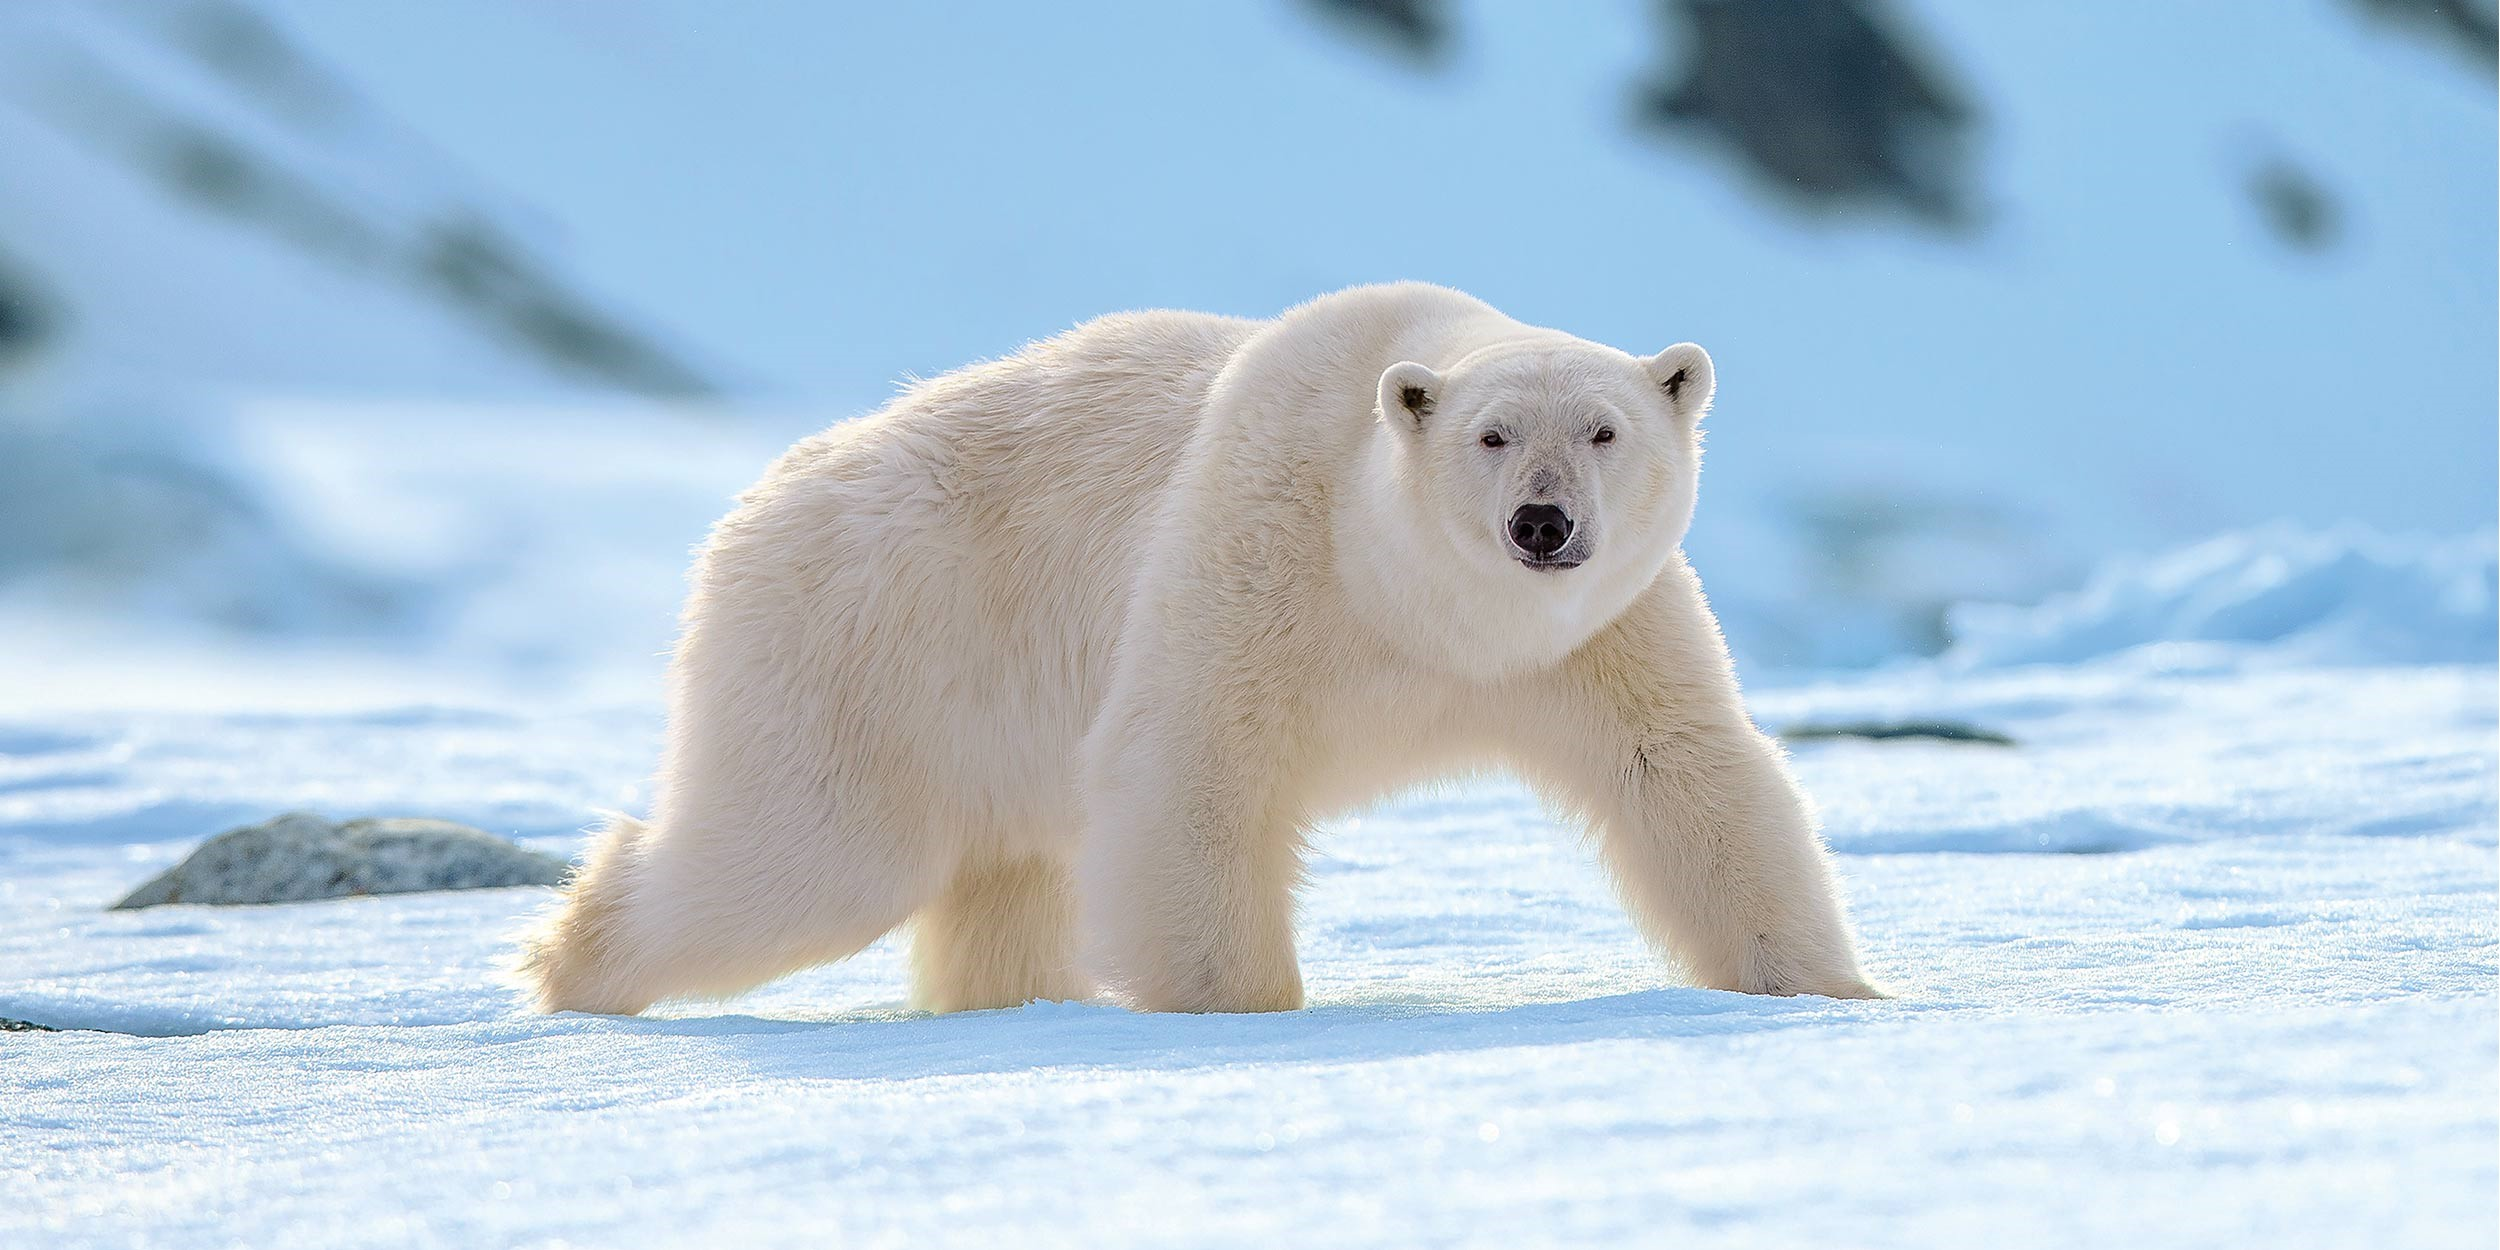
\includegraphics[width=5cm]{example}
    \hfill
    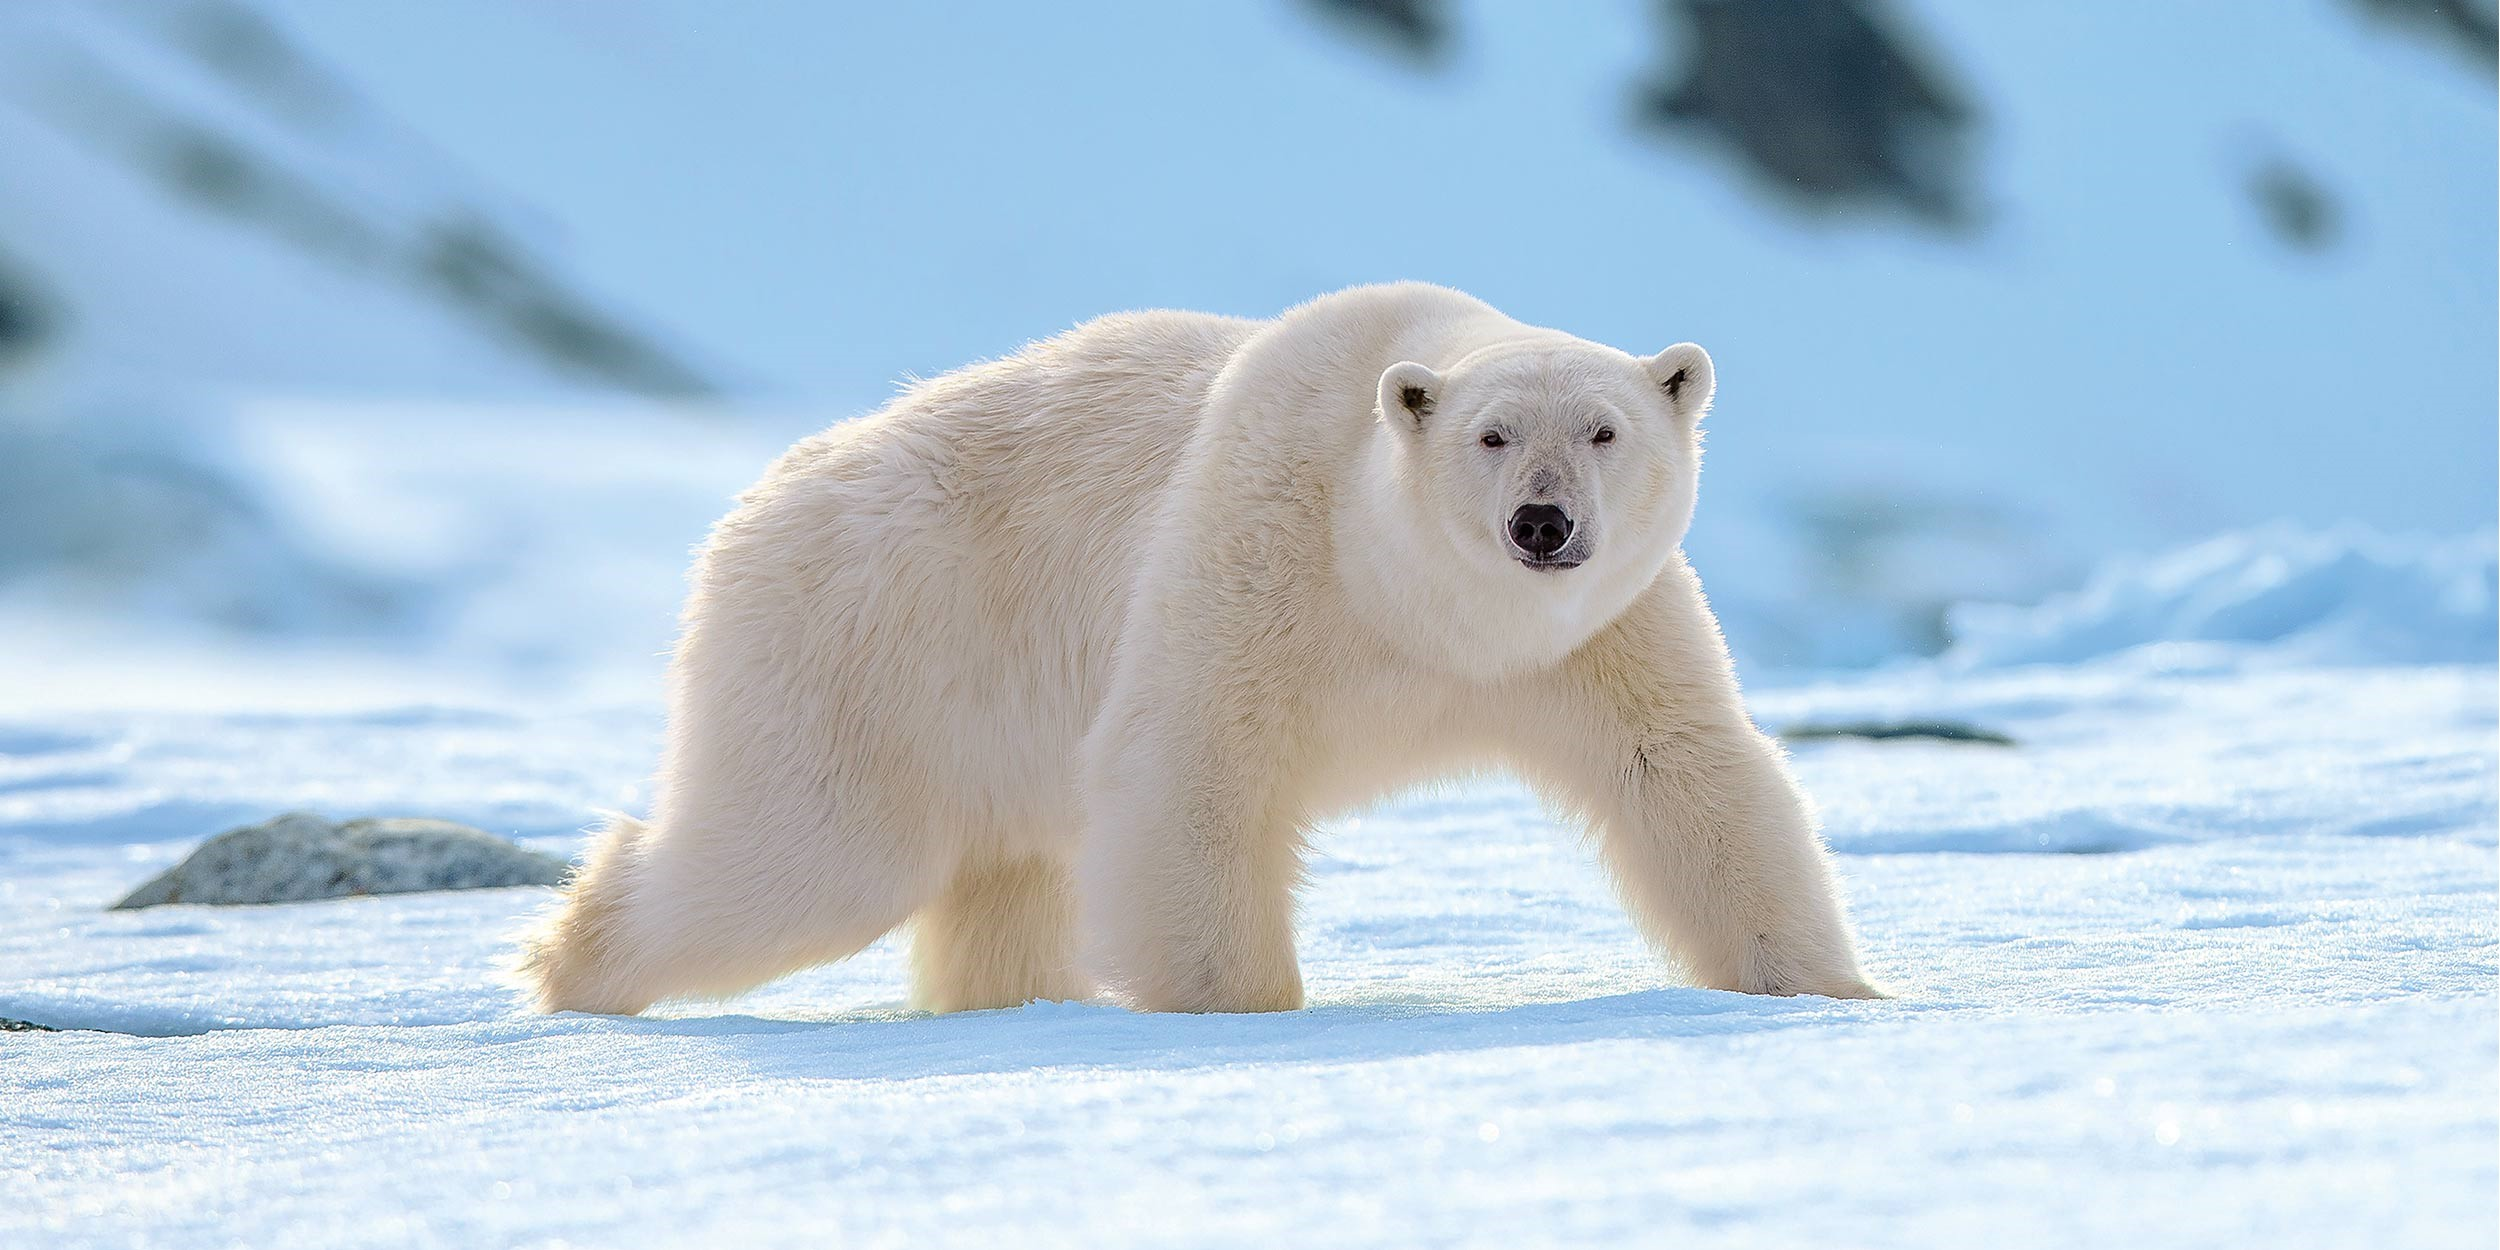
\includegraphics[width=5cm]{example}
    \HRule{13pt}{1pt}
    \centering
    \vlinespace{5}\\
    \workTyp\\
    \begin{Large}
        \textbf{Titel}\\
        \textbf{und mehr}\\
    \end{Large}
    \vlinespace{4}
    im Studiengang\\
    <Studiengang>\\
    am \workDatum\\
    \vlinespace{4}
    vorgelegt von\\
    \begin{Large}
        \textbf{\workNameStudent}\\
    \end{Large}
    \vlinespace{1}
    Matrikelnummer: <12345>
    \vfill
    \raggedright{}
    \HRule{13pt}{1pt} \\
    \titleemph{Erstprüfer:} Prof. <wx>\\
    \titleemph{Zweitprüfer:} Prof. <yz>
\end{titlepage}
   \chapter*{Eidesstattliche Erklärung}

Hiermit versichere ich, die vorliegende Arbeit selbstständig und unter ausschließlicher Verwendung der angegebenen Literatur und Hilfsmittel erstellt zu haben.

Die Arbeit wurde bisher in gleicher oder ähnlicher Form keiner anderen Prüfungsbehörde vorgelegt und auch nicht veröffentlicht.

\begin{tabbing}
          Esslingen, den \workDatum~~\= \rule{5cm}{0.3mm}\\
                                                                                                    \> Unterschrift
\end{tabbing}


   \tableofcontents
   \newpage
   \chapter{Einleitung}\label{sec:motivation}
\section{Hintergrund und Motivation}

Im Rahmen der Arbeit wird eine webbasierte Labeling-Plattform zur Kennzeichnung von KI Daten als Prototyp realisiert. Die Plattform soll das schnelle Labeln von Texten und Bildern ermöglichen. Zum besseren Vergleich der Technologien, wird ein MEVN-Stack verwendet. Dies bietet außerdem den Vorteil, dass der Softwarestack weit verbreitet ist und ein realistisches Anwendungsszenario geschaffen wird.
   \section{Zielsetzung der Arbeit}\label{sec:zielsetzung}
Die Bachelorarbeit zeigt eine Gegenüberstellung von erhältlichen Open-Source Lösungen. Anschließend werden die verschiedenen Technologien in ein eigenes Projekt eingebunden. Das System verwendet einen Menschen zur Beschriftung der Daten. So können die Ergebnisse schneller verifiziert werden und die Komplexität gering gehalten werden. Final können auf der selbsterstellten Webplattform Bilder gekennzeichnet werden. Die Funktionalität, Dokumentation und Simplizität der Komponenten wird genauer beleuchtet.
   \label{sec:aufbau}
\section{Aufbau der Arbeit}

   \newpage
   \chapter{Grundlagen}\label{sec:basics}
\section{Labeling Plattformen: Definition und Bedeutung}\label{sec:basics-labeling-plattformen-definition}

\begin{itemize}
    \item Active learning (AL) (Settles 2009), in which the system remains in control of the
learning process and treats humans as oracles to annotate unlabeled data.
    \item Interactive machine learning (IML) (Amershi et al. 2014), in which there is a closer
interaction between users and learning systems, with people interactively supplying
information in a more focused, frequent, and incremental way compared to traditional
machine learning.
    \item Machine teaching (MT) (Simard et al. 2017; Ramos et al. 2020), where human domain
experts have control over the learning process by delimiting the knowledge that they
intend to transfer to the machine learning model.
\end{itemize}

   \section{Softwarestack: Begriffsdefinition und Komponenten}\label{sec:basics-softwarestack-definition}
MongoDB, Express.js, AngularJS und Node.js. MEAN-Stack-Anwendungen sind flexibel, skalierbar und erweiterbar und machen sie damit zum perfekten Kandidaten für Cloud-Hosting. Dies ist ein fundamentaler Baustein für die Webplattform.\\ 
Der Stack enthält einen eigenen Webserver. Somit kann der Stack einfacher implementiert werden und die Datenbank kann auf Wunsch skaliert werden. Eine MEAN-Anwendung ist so optimiert, dass sie alle Kosteneinsparungen und Leistungsverbesserungen der Cloud nutzt.


\textbf{Zentrale Begriffe definieren - Wie ist die Definition von Softwarestack in der BA. Kann abweichen von Allgemeinen Definition}

   \label{sec:labeling-plattform-anforderungen}
\section{Anforderungen an eine Labeling Plattform}
   \section{Überblick über bestehende Softwarestacks für Labeling Plattformen}\label{sec:labeling-platform-ueberblick-softwarestacks}



   \newpage
   \chapter{Evaluierungskriterien für die Prototypisierungstechnologien}\label{sec:funktionalitaet-features}
\section{Funktionalität und Features}
   \section{Skalierbarkeit und Performance}
   \label{sec:usability}
\section{Benutzerfreundlichkeit und Usability}
   \label{sec:security-datenschutz}
\section{Sicherheit und Datenschutz}
   \label{sec:flexibility-anpassbarkeit}
\section{Flexibilität und Anpassbarkeit}
   \label{sec:unterstuetzung-community}
\section{ Unterstützung und Community}

   \newpage
   \chapter{Analyse und Vergleich relevanter Softwarestacks}\label{sec:stack-a}
\section{Softwarestack A: Vor- und Nachteile}

   \newpage
   \chapter{Fallstudie: Entwicklung einer Labeling Plattform}\label{sec:anforderungsanalyse}
\section{Anforderungsanalyse für die zu entwickelnde Plattform}

Wie weit / abgeschlossen ist die Technologie

Bilder müssen in der gleichen Größe hinterlegt werden. Eine Funktion die Bilder auf den selbigen Bildbereich zuschneiden oder vergrößern zu können, ist unabdingbar.

Daten mit Verzerrungen oder Rauschen müssen extra auf überwacht werden. Es ist sinnvoll eine Möglichkeit zur Verfügung zu stellen, bei der Trainingsdaten mit beschriebenen Merkmalen gekennzeichnet werden können. Eine Fourier-Transformation / Gaußsche Glättung des Signals kann das Rauschen verringern.

Falls möglich, sollten die Freiheitsgrade verringert werden, um unnötige Datenmengen zu verringern. Die Verringerung der Freiheitsgrade muss auf die einzelnen Fälle abgestimmt werden, da ähnliche Elemente nicht mehr erkannt werden können sollte zu sehr generalisiert werden. Ein Beispiel einer zu hohen Verringerung wären einzelne Klassen bei der Buchstabenerkennung (bei n und h).

Für einen möglichst einfachen und natürlichen Weg einen Treffer zu messen, kann die Hamming Distanz verwendet werden (\cite[][]{cv-principles-link}). Eine geringe Hamming Distanz bedeutet, dass eine hohe Übereinstimmung besteht.

Desweiteren können Bilder auch in gedrehter Form gespeichert sein. Dies sorgt für keine Übereinstimmung obwohl die Bilder identisch wären. Zur Vorbeugung können Referentlinien (T beispielsweise eine horizontale und eine vertikale Linie) verwendet werden und die Bilder vorab in die richtige Position gedreht werden.

Außerdem können die Bilder außerhalb des Bildzentrums liegen. Dies erhöht die Freiheitsgrade unnötig. Eine Funktion zum Zentrieren des Bildes ist wünschenswert. 

Einordnen in Gruppierung als Datenpunkt.


Kontrasterhöhung um Bildbereiche/ Elemente besser erkennen zu können.
-> Graustufen Gewichtung:
HDTV Formula ("0.21×Red + 0.72×Green + 0.07×Blue")
PAL/NTSC Formula( "0.30×Red + 0.59×Green + 0.11×Blue")

Link: \url{https://web.s.ebscohost.com/ehost/ebookviewer/ebook/bmxlYmtfXzEyMDQyODlfX0FO0?sid=7eaf4273-b0ca-4e23-af7e-c46da0867380@redis&vid=0&lpid=lp_iii&format=EB}


   \section{Architektur und Design der Plattform}\label{sec:architektur}
   \section{Implementierung und Umsetzung}\label{sec:implementierung}
   \label{sec:testing}
\section{Testing und Validierung}
   \label{sec:herausforderungen}
\section{Erfahrungen und Herausforderungen während der Entwicklung}

   \newpage
   \chapter{Bewertung und Schlussfolgerungen}\label{sec:bewertung}
\section{Bewertung der ausgewählten Softwarestacks anhand der Evaluierungskriterien}
   \label{sec:bewertung-vergleich-anforderungen}
\section{Vergleich der entwickelten Plattform mit den Anforderungen}
    \section{Erkenntnisse und Empfehlungen für die Auswahl zukünftiger Softwarestacks}\label{sec:erkenntnisse}
   \label{sec:fazit}
\section{Fazit und Ausblick}

   \listoffigures
   \renewcommand\lstlistingname{Codefragment}
   \renewcommand\lstlistlistingname{Codeverzeichnis}
   \lstlistoflistings
   \printacronyms[heading=addchap]
   \printnoidxglossary

   \section{Example}

\begin{figure}[H]
    \begin{center} 
        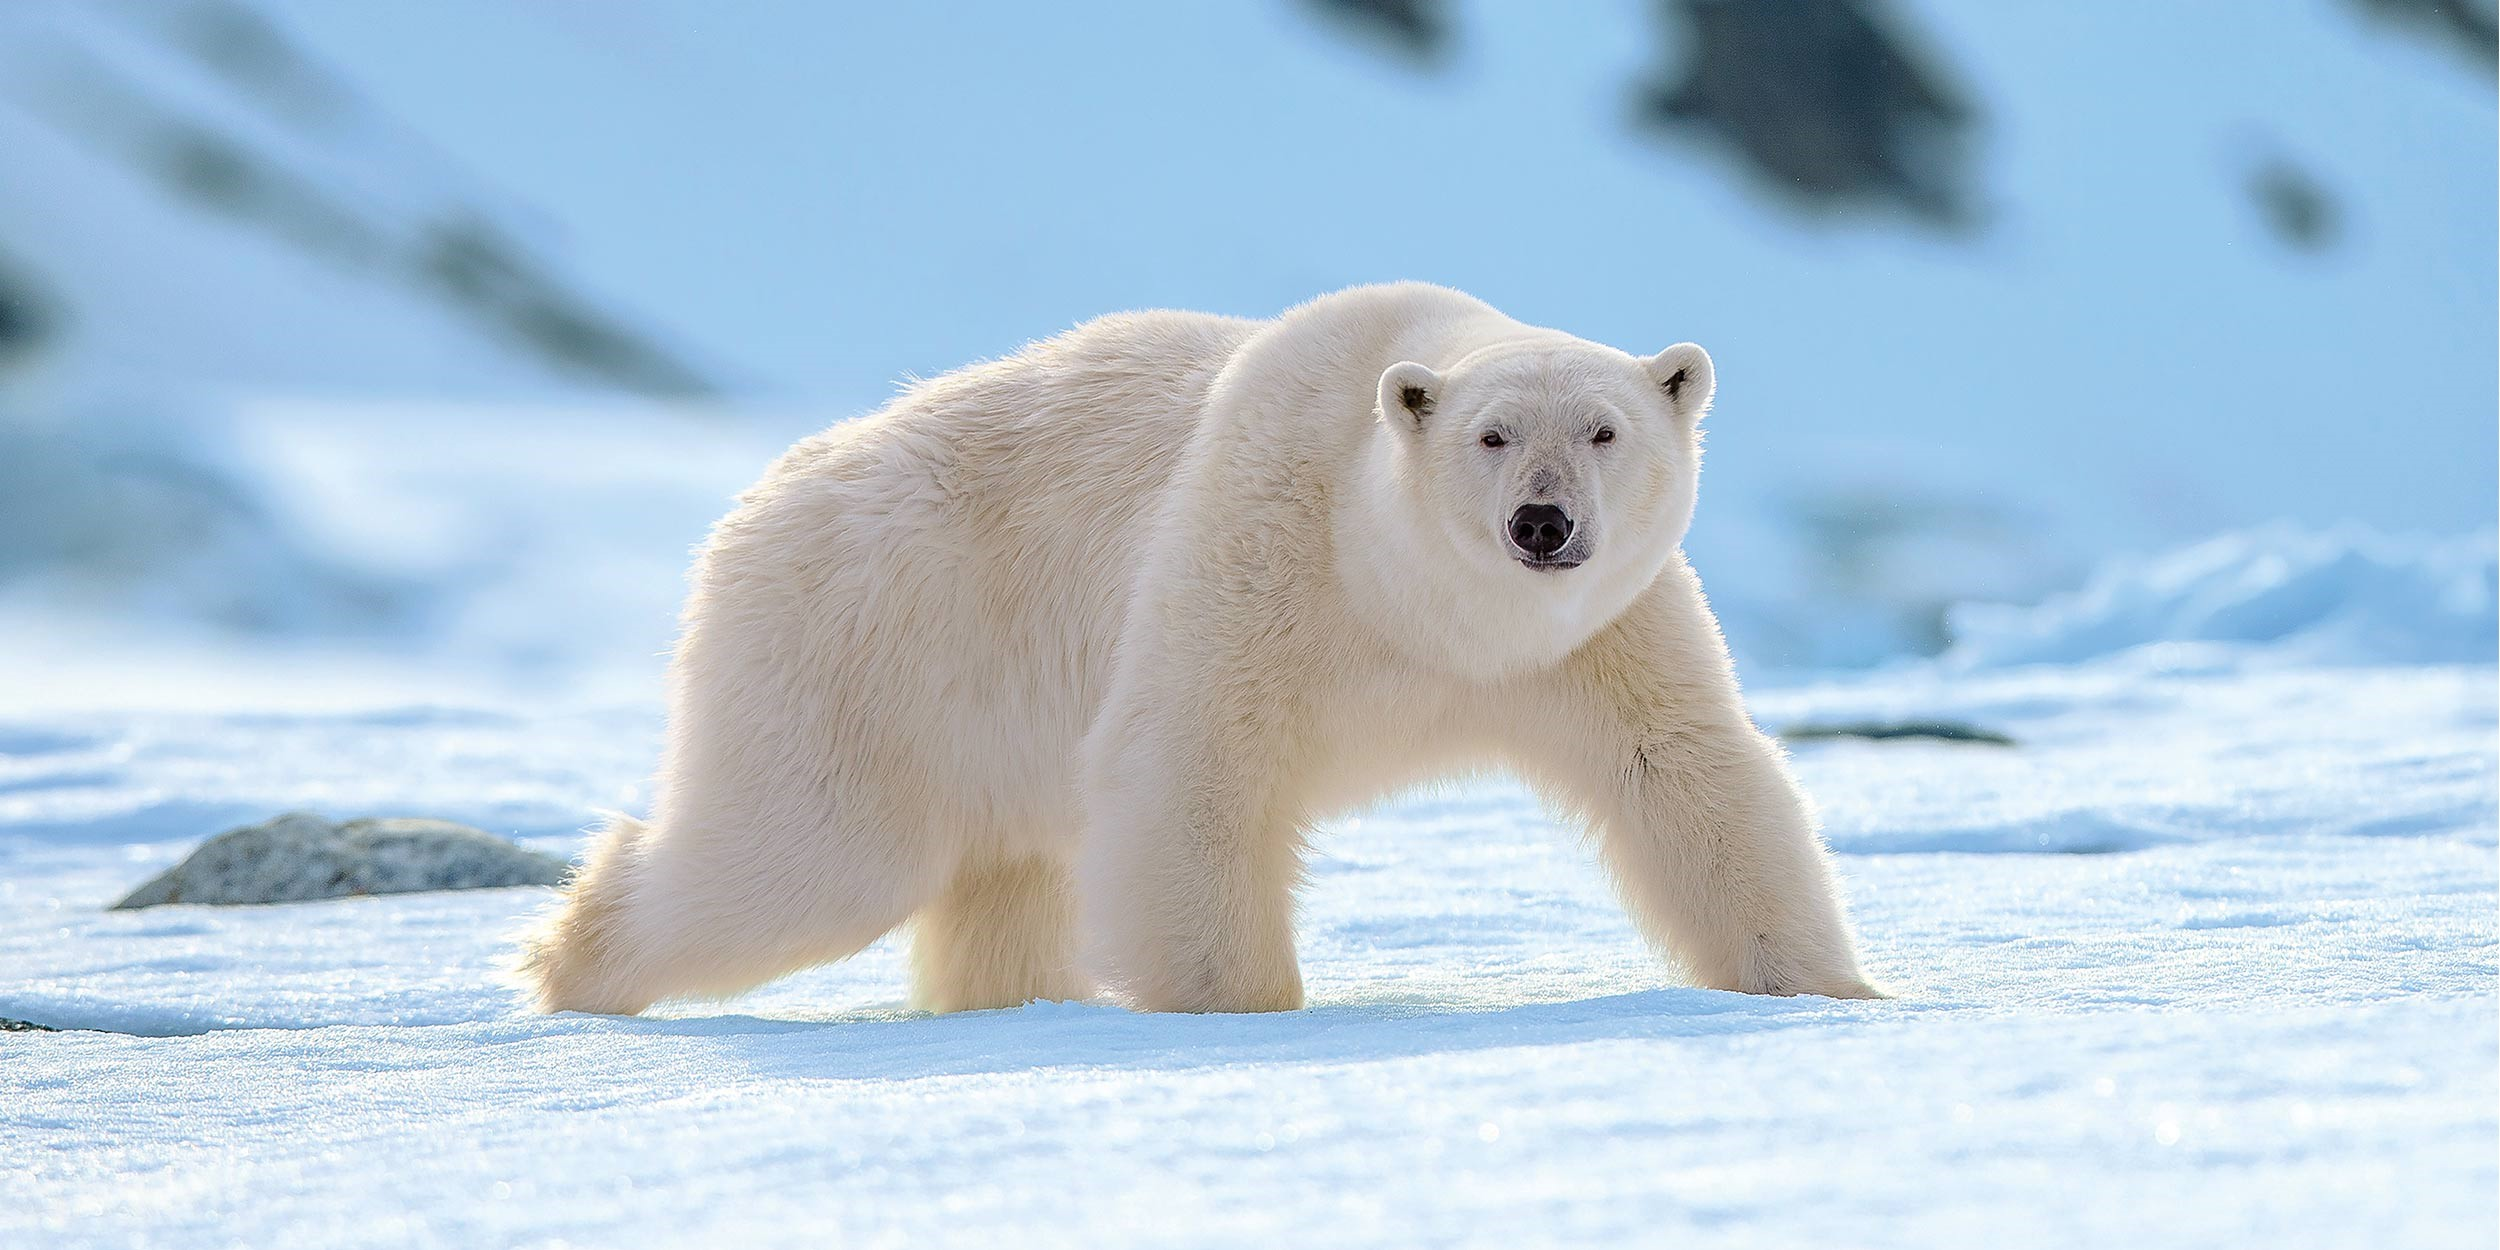
\includegraphics[width=0.8\textwidth]{example}
        \caption{Example Image}
        \label{fig:example}
    \end{center}
\end{figure}

\cite[vgl. dazu][]{example-book}

\cite[vgl. dazu][]{example-online}

\newpage

\begin{lstlisting}[language=Bash]
#!/bin/bash

echo "Hello World"
\end{lstlisting}

\begin{lstlisting}[language=Python]
# same in python

print("Hello World")
\end{lstlisting}

\begin{verbatim}
$ sudo apt-get update
$ sudo apt-get install python
\end{verbatim}

   \chapter{Einleitung} \label{sec:definition}
\section{Definition}
Im Rahmen Deiner Arbeit realisierst Du eine webbasierte Labeling-Plattform zur Kennzeichnung von KI Daten als Prototyp. Die Plattform soll das schnelle Labeln von Texten und Bildern ermöglichen. Um die Entwicklung zu beschleunigen, verwendest Du einen Softwarestack wie MEAN, MERN, MEVN oder JAM. Dies hat vor allem den Vorteil, dass Du zum Start der Entwicklung bereits eine Plattform aus gut zusammenspielenden Softwarekomponenten hast. Die genauen Anforderungen der Abschlussarbeit werden wir gemeinsam mit Dir erarbeiten.

\section{MEAN Stack}
MongoDB, Express.js, AngularJS und Node.js.
MEAN-Stack-Anwendungen sind flexibel, skalierbar und erweiterbar und machen sie damit zum perfekten Kandidaten für Cloud-Hosting. Der Stack enthält einen eigenen Webserver, so dass er einfach implementiert werden kann, und die Datenbank kann auf Wunsch skaliert werden, um temporäre Nutzungsspitzen zu bewerkstelligen. Eine MEAN-Anwendung ist so optimiert, dass sie alle Kosteneinsparungen und Leistungsverbesserungen der Cloud nutzt.

\section{MERN}
MongoDB, Express.js, ReactJS und Node.js.

\section{MEVN}
MongoDB, Express.js, VueJS und Node.js.

\section{JAM}
JavaScript, APIs und Markup

\section{MongoDB}
MongoDB ist eine hoch skalierbare und flexible Dokumentendatenbank mit effizienter Abfrage und Indizierung. MongoDB speichert Daten in flexiblen, JSON-ähnlichen Dokumenten, d. h. Felder können von Dokument zu Dokument variieren und die Datenstruktur kann im Laufe der Zeit geändert werden.

\section{ExpressJS}
Express ist ein minimales und flexibles NodeJS-Webanwendungs-Framework, das robuste Funktionen für Web- und mobile Anwendungen bietet. Es stellt eine Vielzahl von HTTP-Utility-Methoden und Middleware zur Verfügung, mit denen sich schnell und einfach eine robuste API erstellen lässt. Express bietet eine vielfältige Schicht grundlegender Webanwendungsfunktionen.

\section{VueJS}
Laut der Dokumentation ist Vue.js ein progressives JavaScript-Framework für die Erstellung von Benutzeroberflächen. Es ist zugänglich, leistungsfähig und vielseitig bei der Erstellung von Single-Page-Webanwendungen.
VueJS konzentriert sich auf die Ansichtsschicht. Es hat eine sehr einfache Lernkurve mit einer einfachen API, was es zu einem der beliebtesten Frameworks macht.

\section{NodeJS}
Node.js ist eine Open-Source-Laufzeitumgebung und -Bibliothek, die zur Ausführung von Webanwendungen außerhalb des Browsers des Kunden verwendet wird. Sie wird hauptsächlich für die serverseitige Programmierung verwendet. Es ist asynchron, ereignisgesteuert und hoch skalierbar, um Server und Datenbanken zu schreiben.


   \chapter{Wissenschaftliche Vertiefung} \label{sec:research}
\section{Prototypisierung mit Python}
\subsection*{Pillow}
Pillow ist der Nachfolger der Python Imaging Library. Es stellt Funktionen zur Archivierung, Anzeige und Bearbeitung von Bilddateien bereit. 
Mit Pillow können Dateien in ein spezifisches Bildformat konvertiert werden. Dies kann laut Dokumentation (\cite[][]{pillow-documentary}) mit der save-Methode der Image Klasse erreicht werden.

\begin{lstlisting} [caption=Konvertierung einer Datei in ein Bildformat durch Pillow, label=code:pillow-image-converter]
import os, sys
from PIL import Image

for infile in sys.argv[1:]:
    f, e = os.path.splitext(infile)
    outfile = f + ".jpg"
    if infile != outfile:
        try:
            with Image.open(infile) as im:
                im.save(outfile)
        except OSError:
            print("cannot convert", infile)
\end{lstlisting}

Es sind darüber hinaus weitere Bildmanipulationen möglich. Darunter fallen das Ausschneiden eines Bildbereiches, das Einfügen des Ausschnitts in ein anderes Bild oder das Drehen des Bildes. Zur Verbesserung der Bildqualität ist ein ImageEnhance Modul enthalten. Mit diesem kann unter anderem der Kontrast eingestellt werden. Für sequentielle Bildformate, wie FLI, TIFF oder GIF, gibt es eine Funktion die einzelnen Frames einzuladen. Zuletzt verfügt die Pillow Bibliothek über eine PostScript-Unterstützung zum Ausdrucken der Bilddateien. 
Videoformate werden von Pillow nicht unterstützt. Damit sind lediglich die Grundlagen zur Bildmanipulation gegeben.

\subsection*{PyLab}
Interactive annotation. Mit PyLab kann eine Markierung im Bild oder eine Notiz an den Trainingsdaten gesetzt werden.

\begin{lstlisting} [caption=PyLab: Kommentieren einer Datei, label=code:pylab-Interactive-annotation]
from PIL import Image
from pylab import *
im = array(Image.open('empire.jpg'))
imshow(im)
print 'Please click 3 points'
x = ginput(3)
print 'you clicked:',x
show()
\end{lstlisting}

\subsection*{labelImg}
LabelImg is a graphical image annotation tool and label object bounding boxes in images (\cite[][]{labelImg-link}).

\subsection*{Computer Vision Annotation Tool }
CVAT is an interactive video and image annotation tool for computer vision. It is used by tens of thousands of users and companies around the world. Our mission is to help developers, companies, and organizations around the world to solve real problems using the Data-centric AI approach. (\cite[][]{CVAT-link}).

\subsection*{labelme}
Image Polygonal Annotation with Python (\cite[][]{labelme-link}).
Labelme is a graphical image annotation tool inspired by http://labelme.csail.mit.edu.
It is written in Python and uses Qt for its graphical interface.

\subsection*{VoTT}
An open source annotation and labeling tool for image and video assets.
VoTT is a React + Redux Web application, written in TypeScript. This project was bootstrapped with Create React App. (\cite[][]{VoTT-link})
\textbf{VoTT is no longer being maintained!}

\subsection*{imglab}
A web based tool to label images for objects that can be used to train dlib or other object detectors. (\cite[][]{imglab-link})

\subsection*{PixelAnnotationTool}
Software that allows you to manually and quickly annotate images in directories. The method is pseudo manual because it uses the algorithm watershed marked of OpenCV. The general idea is to manually provide the marker with brushes and then to launch the algorithm. If at first pass the segmentation needs to be corrected, the user can refine the markers by drawing new ones on the erroneous areas (\cite[][]{PixelAnnotationTool-link}).


Bilder können mit Hilfe von NumPy als Array repräsentiert werden. NumPy bietet vielfältige Möglichkeiten Daten zu speichern. Mittels einigen Konvertiermethoden lässt sich der Input und Output besser Verwalten als in andere Bibliotheken. So können im Vorfeld die Ausnahmen konfiguriert werden. Anschließend kann die Konvertierung automatisiert durchgeführt werden.
Darüber hinaus gibt es Transformationsmöglichkeiten für Vektoren.


- datasets for labeling CV
- timeserious daten labelin
nest js
Umsetzung eines Softwarestacks
(analyse)
zeitplan -> kick off mit koch

\subsection*{Zeitplan / Exposé}
\subsubsection*{Orientierungs- und Planungsphase}
\begin{itemize}
    \item Thema finden (Auswahl eines geeigneten Softwarestacks für die Entwicklung einer Labeling Plattform) \textbf{DONE}
    \item Fragestellung und vorläufige Gliederung \textbf{Bis 12.09.23 / nach Besprechungstermin Koch}
    \item Passende Literatur recherchieren und sichten \textbf{Bis 17.09.23}
\end{itemize}

\subsubsection*{Recherche- und Materialbeschaffungsphase}
\begin{itemize}
    \item Intensive Literatursuche und -analyse \textbf{Bis 15.10.23}
    \item Forschungsdesign auswählen und vertiefen \textbf{Bis 1.11.23}
    \item Daten sammeln \textbf{Bis 15.11.}
    \item Datenanalyse und -auswertung \textbf{Bis 20.11.23} 
\end{itemize}


\subsubsection*{Schreibphase}
    \begin{itemize}
        \item Einleitung, Literaturübersicht, Fazit \textbf{Bis 13.12.23}
    \end{itemize}

\subsubsection*{Abschlussphase}
\begin{itemize}
    \item Korrektur, Layout \textbf{Bis 10.01.24}
    \item Druck, finaler Schliff \textbf{Bis 19.01.24}
\end{itemize}

\section{Prototypisierung mit JS}
nestjs: Alternative zu Express. Nest bietet eine sofort einsatzbereite Anwendungsarchitektur, die es Entwicklern und Teams ermöglicht, hochgradig testbare, skalierbare, lose gekoppelte und leicht wartbare Anwendungen zu erstellen. Die Architektur ist stark von Angular inspiriert

\subsection*{SciPy}
Image Derivate: Dabei werden die x- und y-Ableitungen und die Gradientengröße mit Hilfe des Sobel-Filters berechnet. 
In SciPy.IO ist es möglich matLab Dateien zu laden.


\subsection*{Morphologie}
mehrere datensätze 9088

\subsection*{Mögliche Datensätze}
\begin{itemize}
    \item World University Ranking 2023 (\url{https://www.kaggle.com/datasets/alitaqi000/world-university-rankings-2023})
\end{itemize}


   \printbibheading[title=Literaturverzeichnis]
   \printbibliography[type=book,heading=subbibliography,title=Buch-Quellen]
   \printbibliography[type=online,heading=subbibliography,title=Online-Quellen]

\end{document}